\documentclass[UTF8]{article}


% if you need to pass options to natbib,use,e.g.:
%     \PassOptionsToPackage{numbers,compress}{natbib}
% before loading neurips_2022


% ready for submission
\usepackage[final]{neurips_2022_zh}

% \PassOptionsToPackage{numbers,compress}{natbib}


% to compile a preprint version,e.g.,for submission to arXiv,add add the
% [preprint] option:
%     \usepackage[preprint]{neurips_2022}


% to compile a camera-ready version,add the [final] option,e.g.:
%     \usepackage[final]{neurips_2022}


% to avoid loading the natbib package,add option nonatbib:
%    \usepackage[nonatbib]{neurips_2022}

\usepackage{ctex} % support zh
\usepackage{indentfirst} %support indent
\usepackage{graphicx} % support image
\usepackage[colorlinks, linkcolor=blue]{hyperref}
\usepackage[utf8]{inputenc} % allow utf-8 input
\usepackage[T1]{fontenc}    % use 8-bit T1 fonts
\usepackage{hyperref}       % hyperlinks
\usepackage{url}            % simple URL typesetting
\usepackage{booktabs}       % professional-quality tables
\usepackage{amsfonts}       % blackboard math symbols
\usepackage{nicefrac}       % compact symbols for 1/2,etc.
\usepackage{microtype}      % microtypography
\usepackage{xcolor}         % colors

\setlength{\parindent}{2em}
\title{动态本地可搜索对称加密}


% The \author macro works with any number of authors. There are two commands
% used to separate the names and addresses of multiple authors: \And and \AND.
%
% Using \And between authors leaves it to LaTeX to determine where to break the
% lines. Using \AND forces a line break at that point. So,if LaTeX puts 3 of 4
% authors names on the first line,and the last on the second line,try using
% \AND instead of \And before the third author name.


\author{%
  肖泽宇\thanks{本文是对Crypto2022 "Dynamic Local Searchable Symmetric Encryption"的翻译}\thanks{参考原文链接 https://hal.archives-ouvertes.fr/hal-03863896/document} \\
  \texttt{2022202210145} \\
  % examples of more authors
  % \And
  % Coauthor \\
  % Affiliation \\
  % Address \\
  % \texttt{email} \\
  % \AND
  % Coauthor \\
  % Affiliation \\
  % Address \\
  % \texttt{email} \\
  % \And
  % Coauthor \\
  % Affiliation \\
  % Address \\
  % \texttt{email} \\
  % \And
  % Coauthor \\
  % Affiliation \\
  % Address \\
  % \texttt{email} \\
}


\begin{document}


\maketitle


\begin{abstract}
  在这篇文章中,我们将首次解决动态内存高效的可搜索对称加密问题(SSE)。这里的术语“内存高效”包括local内存高效和页内存高效。我们方法的核心是在这两个目标之间建立一种新型的联系。我们引入了一个被称为泛型局部变换的映射,它将具有某些特殊特征的高效页SSE方案作为输入,并输出具有强局域性的SSE方案。我们得到了以下几个结果。
  \begin{itemize}
    \item 首先,对于页面高效SSE,我们构建了一个页面效率O(log log N)和存储效率O(1)的动态方案,称为LayeredSSE。LayeredSSE背后的主要技术创新是两个选择分配过程的一个新的加权扩展,具有独立的利益。TODO
    \item 其次,引入泛型局部变换,并将其与LayeredSSE相结合,在最长列表大小为$\mathcal{O}\left(N^{1-1 / \log \log \lambda}\right)$的条件下,构建存储效率O(1),局域性O(1),读取效率O(log log N)的动态SSE方案。这在各方面都与Asharov等人在STOC 2016上提出的纯静态结构相匹配:动态性无需额外成本。
    \item 最后,通过将通用局部变换应用于Bossuat等人从Crypto 2021提出的Tethys方案的变体,我们构建了一个无条件静态SSE,其存储效率O(1), localityO(1),读取效率$\mathcal{O}\left(\log ^{\varepsilon} N\right)$,对于任意小的常数$\varepsilon$ > 0。据我们所知,这是Cash和Tessaro在2014年Eurocrypt上提出的最接近下限的结构。
  \end{itemize}
\end{abstract}


\section{简介}
\textbf{可搜索对称加密。}在可搜索对称加密(SSE)中,客户端将一组文档的存储托管给不受信任的服务器。客户端希望具备通过向服务器发出搜索请求来执行搜索的能力。在动态SSE的设置中,客户端还可以发出更新请求,以便修改文档的内容,例如添加或删除条目。服务器必须能够正确地处理所有请求,同时尽可能少地了解文档数据和请求的信息。SSE与许多云存储场景相关:例如,在托管敏感数据库或提供加密消息传递服务等情况下,可能非常需要某种形式的搜索功能。

理论上,SSE是加密数据计算的一种特殊情况,可以使用通用的解决方案来实现,例如完全同态加密。但在实践中,这种方法会导致很大的性能损失。因此,SSE方案通常以高性能解决方案为目标,可扩展到大型真实场景数据库。为此,SSE不惜以安全换取效率。服务器被允许了解一些关于客户端数据的信息。例如,SSE方案通常向服务器泄漏查询的重复(搜索模式)和与查询匹配的文档标识符(访问模式)。SSE的安全模型通过泄漏函数进行参数化,该函数描述泄漏给服务器的信息的性质。

\textbf{位置。}在单关键字SSE的情况下,搜索查询要求包含给定关键字的所有文档。为了实现该功能,服务器维护一个(加密的)反向索引,其中每个关键字都映射到与关键字匹配的文档标识符列表。当客户希望搜索与给定关键字匹配的文档时,客户只需从服务器检索相应的列表。然而,一个关键的问题是服务器应该如何存储和访问列表。

一个列表接一个列表存储的简单方法并不令人满意:实际上,给定列表在内存中的位置依赖于其他列表的长度,从而泄露了关于这些列表的信息。解决这个问题的常用方法是将每个列表元素存储在内存中的随机位置。在这种情况下,当检索列表时,服务器必须访问与列表中元素数量一样多的随机内存位置。这也是不可取的,原因不同:对于几乎所有的现代存储介质,访问许多随机内存位置比访问一个连续区域要昂贵得多。由于SSE依赖于快速对称密码原语,内存访问成本成为性能瓶颈。为了获取成本,\cite{DavidCash2014TheLO}引入了局部性的概念:简而言之,SSE方案的局部性是服务器必须访问以回答查询的不连续内存位置的数量。

上面概述的两个极端解决方案表明安全性和局部性之间存在冲突。在Eurocrypt 2014年,Cash和Tessaro表明这种冲突是固有的\cite{DavidCash2014TheLO}:如果安全SSE方案具有恒定的存储效率(加密数据库的大小与明文数据库的大小成线性关系)和恒定的读取效率(服务器为回答搜索查询而读取的数据量与明文答案的大小成线性关系),那么它不可能具有恒定的局域性。

\textbf{本地SSE结构。}从那时起,许多具有定域性的SSE方案被提出,通常是以超常读效率为代价的。在STOC 2016上,Asharov等人提出了一种具有O(1)存储效率、O(1)局部性和O(log N)读取效率的方案,其中N是数据库的大小\cite{GiladAsharov2021SearchableSE}。在Crypto 2018上,Demertzis等人将读取效率提高到$\mathcal{O}\left(\log ^{2 / 3+\varepsilon} N\right)$\cite{IoannisDemertzis2018SearchableEW}。在\cite{IoannisDemertzis2017FastSE}中还提出了$\omega$(1)存储效率的一些权衡。当数据库中最长列表的大小受到限制时,就会得到更强的结果。当需要这样一个上界时,我们将该构造称为有条件的。第一个条件SSE来自于Asharov等人,在最长列表大小为$\mathcal{O}\left(N^{1-1 / \log \log N}\right)$的条件下,达到了O(log log N)个读效率。后来改进为O(log log log N)读取效率,在最长列表的大小上有更强的条件$\mathcal{O}\left(N^{1-1 / \log \log \log N}\right)$。

局部性被引入作为内存访问的性能度量,假设在硬盘驱动器上实现。在\cite{AngleBossuat2021SSEAS}中,Bossuat等人表明,在固态硬盘(如闪存盘)的情况下,局部性不再是相关的目标。相反,性能主要取决于访问的内存页的数量,而不管它们是否连续。在这种情况下,正确的性能指标是页面效率。页面效率定义为服务器为回答查询而读取的页面数,除以存储明文答案所需的页面数。\cite{AngleBossuat2021SSEAS}的主要结构实现了O(1)存储效率和O(1)页效率,假设客户端内存为$\omega$(log λ)页。

到目前为止,所有现有结构(包括本地结构和页面高效结构)的一个共同点是它们都是纯静态的。这可能是因为构建局部SSE固有的困难,即使是在静态情况下(从一开始,Cash和Tessaro的不可能性结果就证明了这一点\cite{DavidCash2014TheLO})。然而,SSE的许多(如果不是大多数的话)应用程序需要动态性。这种情况严重阻碍了本地高效的SSE的适用性。
\subsection{我们的贡献}
在本文中,我们首次考虑了动态内存高效SSE的问题,这意味着我们同时针对动态页面高效SSE和动态局部高效SSE。我们方法的核心是在这两个目标之间建立一种新颖的联系。我们引入了一个称为泛型局部变换的映射,它将具有某些特殊特征的高效页SSE方案作为输入,并输出具有强局域性的SSE方案。我们的策略将是首先构建高效页面的方案,然后应用泛型局部变换获得局部方案。这种方法被证明是相当有效的,我们给出了几个结果。\ref{table1} \ref{table2}
\begin{figure}[ht]
  \centering
  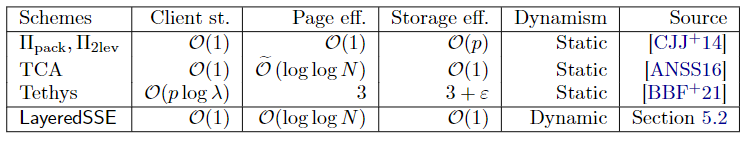
\includegraphics[scale=0.5]{table1.png}
  \caption{高效页面SSE方案。N表示数据库的总大小,p是每页元素的数量,$\varepsilon$ > 0是一个任意小的常数,$\lambda$ 是安全参数。页面效率、存储效率和客户端存储在章节3.1.2中定义。}
  \label{table1} %这样,就可以通过~\ref{fig_1}引用图片了
\end{figure}

\begin{figure}[ht]
  \centering
  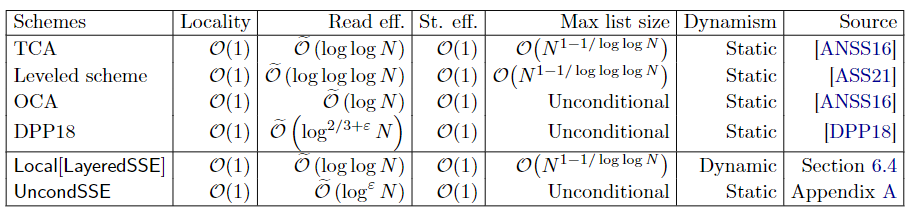
\includegraphics[scale=0.4]{table2.png}
  \caption{具有定域性和存储效率的SSE方案。N表示数据库的总大小,$\varepsilon$ > 0是一个任意小的常数。局部性、读效率和存储效率的定义见章节3.1.2。}
  \label{table2} %这样,就可以通过~\ref{fig_1}引用图片了
\end{figure}

\begin{itemize}
  \item \textbf{动态高效页面SSE。}我们首先构建一个动态页面高效SSE方案LayeredSSE。LayeredSSE实现存储效率O(1),页面效率O(log log N)。与之前关于内存高效SSE的工作一致,LayeredSSE的技术核心是一种新的动态分配方案L2C。L2C是所谓的“2-choice”算法的加权变体,在资源分配文献中臭名昭著。(更多细节在技术概述中提供。)因此,L2C具有独立的利益。
  \item \textbf{泛型局部变换。}我们将介绍泛型局部变换。在输入任何具有特定特征的页效率方案PE-SSE时,称为页长隐藏SSE,通用局部变换输出一个局部SSE方案Local[PE-SSE]。粗略地说,如果PE-SSE有客户端存储O(1),存储效率O(1),页面效率O(P),那么Local[PE-SSE]的存储效率O(1),读取效率O(P)。关于局部性,关键特征是如果PE-SSE在查询最多一个页面大小的列表时具有局部性O(L),那么Local[PE-SSE]在查询任何大小的列表时具有局部性O(L + log log N)。因此,局部构造可以看作是将具有弱局部性的方案引导到具有强得多的局部性的方案。
  
  泛型局部转换还强调了页面效率和局部性目标之间的有趣联系。最初,局部性和页面效率作为不同的性能标准被引入,分别针对两种最广泛的存储介质:硬盘驱动器和固态驱动器。在\cite{AngleBossuat2021SSEAS}中已经观察到,具有局部L和读效率R的方案必须具有最多R + 2L的页效率。从这个意义上说,页面效率是一个“更容易”的目标。令人惊讶的是,使用泛型局部变换,我们在相反的方向上构建了一个连接:我们使用高效页面方案作为构建块来获得局部方案。理论上讲,这显示了两个目标之间的强烈联系。在实际层面上,它提供了同时实现这两个目标的策略。
  \item \textbf{动态本地SSE。}通过将通用局部变换应用于LayeredSSE页效率方案,我们立即获得了一个动态SSE方案Local[LayeredSSE],其存储效率O(1),局域性O(1),读取效率O(log log N)。构造是有条件的:它要求最长列表的大小为$\mathcal{O}\left(N^{1-1 / \log \log N}\right)$。Local[LayeredSSE]的渐近性能与[ANSS16]的第二个静态结构完全匹配,包括最大列表大小的条件:动态不需要额外的代价。特别是,Local[LayeredSSE]匹配[ASS21]中SSE方案的下界,使用[ASS21]称为“分配方案”构建,这表明即使在动态设置中也可以匹配边界。
  \item \textbf{静态设置中无条件的本地SSE。}来自[ANSS16]的原始1-choice方案无条件地实现O(1)存储效率,O(1)局部性和O(log N)读取效率。在[DPP18]中,对于任意常数ε > 0,读取效率提高到$\mathcal{O}\left(\log ^{2 / 3+\varepsilon} N\right)$。这是迄今为止唯一一个无条件实现亚对数效率的SSE建设。通过将泛型局部变换应用于Tethys的变体[BBF+21],并结合[DPP18]启发的技术,我们获得了一个无条件静态SSE方案,对于任何常数ε > 0,它具有存储效率O(1),局域性O(1)和读取效率$\mathcal{O}\left(\log ^{\varepsilon} N\right)$。据我们所知,这是最接近Cash和Tessaro的不可能结果的结构,它表明O(1)局部性、存储效率和读取效率同时是不可能的。
\end{itemize}

\textbf{关于向前安全的说明。}在这项工作中构建的SSE方案在搜索过程中有一个标准的“最小”泄漏剖面:即搜索泄漏搜索模式和访问模式。对于我们的动态方案,更新操作会泄漏正在更新的列表的标识符,在某些情况下还会泄漏列表的长度。因此,我们的动态方案不是前向安全的。潜在的问题是前向安全性和内存效率的目标似乎从根本上是不一致的。事实上,局部性要求与相同关键字相关联的标识符必须彼此靠近地存储;向前-隐私要求插入新标识符的位置应该独立于与其关联的关键字。这个问题已经在[Bos16]中提到了,他声称“对于动态方案,局部性和前向隐私是两个不可调和的概念”。我们建议读者参考[Bos16]以获得关于该问题的更多讨论。我们把对这个问题的进一步分析留给以后的工作。
\section{技术概述}
这项工作包含几个结果,由泛型局部转换连接在一起。因此,我们认为将它们放在一篇论文中是有益的。这就需要引入一些不同的分配机制。我们努力在本节中对这些机制作一个清楚的概述。形式化的规范、定理和证明将在后续章节中介绍。

首先回顾一些经过充分研究的分配机制是有帮助的。在接下来的内容中,“具有压倒性的概率”等同于“除了可忽略不计的概率”(在通常的密码学意义上),而“具有高概率”仅仅意味着在某种意义上概率接近1,但不一定是压倒性的。

一个选择分配。在单选分配中,n个球被扔进n个箱子。每个球被插入一个独立且均匀随机选择的箱子(通过哈希球的标识符)。使用切尔诺夫边界的标准分析表明,在插入过程的结果中,加载最多的bin包含O(log n)个球,具有高概率[JK77]。(对于任意f = ω(1),绝大多数概率最多有O(f (n) log n)个球。)

两个网络分配。同样,n个球被扔进n个箱子。对于每个球,两个箱子被独立且均匀地随机选择(例如通过哈希一个球的标识符)。在插入球的时候,球被插入两个箱子中含有最少的球。Azar等人的一个著名结果表明,在插入过程的结果中,加载最多的bin包含O(log log n)个球,概率很高[ABKU94]。(后来证明该结果以压倒性的概率成立[RMS01]。)

布谷鸟散列。布谷鸟哈希是由Pagh和Rodler [PR04]引入的一种经典哈希方案。它在密码学中有许多应用:其中,无关算法(cf. [CGLS17],以及其中的引用),私有集交集[PSSZ15],以及最近的可搜索加密[PPYY19,BBF+21]。在布谷鸟哈希中,n个球被插入到(2 + ε)n个单元中,其中ε > 0是一个任意小的常数。每个格子最多可以容纳一个球。对于每个球,两个单元格被独立且均匀地随机选择(例如通过哈希球的标识符)。球被插入两个细胞中的一个。如果该单元已经被占用,则占用的球被移动到其他可能的目标单元,可能会产生连锁反应。Pagh和Rodler已经证明了插入在预期do (log n)时间内终止[PR04](包括在插入失败的情况下,用一个新的哈希函数重建整个表的平摊代价)。最后,类似于二选一分配,每个球被存储在两个可能的位置之一。由于更复杂的插入算法(允许移动已经放置的球),负载最多的单元格(根据定义)的负载为1,而不是O(log log n)的两种选择分配。为了实现可以忽略不计的失败概率,加密应用程序通常使用带有隐藏的布谷鸟哈希[KMW10]。
\subsection{分层的两种选择分配}
我们的第一个目标是构建一个动态页面高效方案。让我们从静态情况开始,总结一下这需要什么。正如在介绍中所解释的,要实现单关键字SSE,我们希望在不受信任的服务器上存储任意大小的列表。可以使用对称加密以一种简单的方式来隐藏列表的内容。主要的挑战是如何将列表存储在服务器内存中,以这样一种方式访问一个列表不会显示关于其他列表长度的信息。

在页面效率方案的情况下,这个挑战可以总结如下。我们有一组列表,总共包含N个项目。我们还得到了一个页面大小p,它表示一个物理内存页面中可以容纳的项的数量。服务器的内存被视为一个页面数组。我们希望将列表存储在服务器内存中,考虑到三个目标。

\begin{enumerate}
  \item 为了存储所有列表,我们总共使用S⌈N/p⌉页的服务器内存,其中S称为分配方案的存储效率。我们想让S尽可能小。
  \item 任何长度为ℓ的列表都可以通过访问服务器内存中最多P个⌈ℓ/ P个⌉的页面来检索,其中P称为分配方案的页面效率。我们希望P尽可能小。
  \item 最后,服务器为检索给定列表而访问的页面不应该依赖于其他列表的长度。
\end{enumerate}

前两个目标正是箱子装箱算法的目标。第三个目标是安全目标:它规定服务器执行的内存访问模式不应该泄露某些信息。因此,目标涉及到无关的或数据独立的算法。在[BBF+21]中,实现这三个目标的框架被形式化为数据独立包装(DIP)。

为了便于表示,我们将关注所有列表的大小最多为一页的情况。如果一个列表的长度超过一页,一般的想法是它将被分割成一页的块,加上最后一个最多一页的块;然后,每个块将被分配方案视为一个单独的列表。我们假设从现在开始列表的长度小于一页。

简而言之,[BBF+21]提出的实例化DIP方案的想法是使用杜鹃哈希的加权变体。更详细地说,对于每个列表,通过散列列表的标识符,统一随机地选择两个页面。然后,列表的每个元素将存储在两个指定页面中的一个页面中,或一个stash中。隐藏存储在客户端。为了选择每个列表如何在其三个可能的目的地(两个选择的页面,或存储)之间分割,[BBF+21]使用了最大流量算法。这个算法的细节与我们的目的无关。重要的一点是,在检索列表时,服务器访问两个统一随机的页面。显然,这不会向服务器透露关于其他列表长度的信息。由此产生的算法,称为Tethys,实现了存储效率O(1),页面效率yo(1),客户端存储ω(log λ)页(用于存储隐藏)。

在本文中,我们希望建立一个动态SSE。为此,底层分配方案需要允许新的更新操作。更新操作允许客户端向列表中添加一个新项,将其长度增加1。安全性目标本质上与静态情况相同:算法为了更新给定列表而访问的页面不应该依赖于其他列表的长度。

Tethys不适合作为动态方案的基础,因为它不支持有效的与数据无关的更新过程:在更新期间向单元格插入元素时,更新过程需要访问其他单元格,其访问模式本质上是与数据相关的。相反,一个自然的想法是使用两种选择分配方案的加权变体。使用两种选择分配,更新期间的访问模式很简单:只需要读取与正在更新的列表关联的两个目标桶。然后将新项插入到当前包含较少项的两个桶中。

实例化该方法将需要一个二选一分配的加权变体,如下所示:给定一个多集列表大小{ℓi: 1≤i≤k},ℓi≤p和∑ℓi = N,在二选一分配过程的结果为O(N/p)个桶时,加载最多的桶以压倒性的概率包含O(p log log N)个项目。然而,这种形式的结果似乎是一个长期存在的开放问题(一些相关的部分结果在[BFHM08]中讨论)。文献[TW07, TW14]中已经研究了加权项目的二选一过程,但据我们所知,所有现有的结果都假设球的重量取样相同且独立于足够平滑的分布。即使不考虑分布上的约束,在我们的设置中,我们甚至不能假设列表长度是独立绘制的:在SSE安全模型中,列表是由对手任意选择和更新的。

为了我们的目的,我们需要一个无分布的陈述:我们只知道每个列表大小的边界p,以及所有列表总大小的边界N。我们想要一个O(p log log N)加载最多的桶大小的上限,它适用于满足这些约束的任何一组列表大小。这种形式的结果是已知的一种选择分配过程[BFHM08](具有O(p log N)上限),但同一篇文章表明,相同的技术不能扩展到两种选择过程。

为了解决这一问题,我们引入了一种分层加权二选择分配算法L2C。L2C具有与(加权)二选算法相同的基本行为:对于每个球,均匀随机地选择两个箱子作为可能的目的地。唯一的区别是如何在两个目标箱子中选择实际插入球的箱子。最自然的选择是将球存储在当前负载最小的容器中,其中容器的负载是当前所包含的球的重量之和。相反,我们使用一个稍微复杂一点的决策过程。简而言之,我们将球的可能权重划分为O(log log λ)子区间,并对每个子区间内的球独立执行决策过程。对于第一个子区间(保留最小的权重),我们使用加权的单选过程,而对于其他子区间,我们使用未加权的二选过程。

这种结构的要点在于,它的分析可以简化为加权的一项选择过程和非加权的两项选择过程的分析,这两项选择过程以强大的分析技术而闻名。我们利用这些技术来证明L2C在负载最多的bin的负载上实现了所需的无分布保证。在实践中,这意味着我们有一个分配算法,在大多数意图和目的下,表现得像二选一分配的加权变体,并且可以相对轻松地获得无分配保证。多项选择分配过程在计算机科学的某些领域普遍存在,这使得它成为独立利益的结果。

LayeredSSE方案是通过在L2C之上增加一层加密和密钥管理,使用SSE文献中的标准技术来获得的,尽管需要注意更新。详情请参阅第5.2节。


\subsection{泛型局部变换}
在Crypto 2018上,Asharov等人确定了构建本地SSE的两个主要范例[ASS18]。第一个是分配范式,它通常使用多项选择分配方案的变体,或布谷鸟哈希法。第二种是“垫-拆”方法。高效内存SSE的主要困难在于将不同大小的列表打包在一起。填充和分割方法的思想是根据列表的大小分别存储列表,从而避免了这个问题。实现这一点最简单的方法是填充所有列表的长度到下一个2的幂。这将产生log N个列表长度的可能值。所有给定长度的列表都可以存储在一起,例如,使用标准哈希表。由于我们不想透露每种长度的列表的数量,因此每一层的哈希表都需要进行维数划分,以便能够接收整个数据库。因此,基本的“垫-拆”方案的存储效率为O(log N),但很容易实现O(1)局部性和读取效率。

对于泛型局部变换,我们引入了溢出SSE (OSSE)的概念。OSSE在所有方面都像SSE方案,除了在其设置和更新期间,它可能拒绝存储一些列表元素。这样的元素称为溢出。OSSE打算用作overaching SSE构造中的子组件。OSSE方案用于存储部分数据库,而溢出元素则使用单独的机制存储。OSSE的概念之前并没有形式化,但事后看来,OSSE的使用可能被视为隐含在几个现有的结构中[DPP18, ASS18, BBF+21]。为了便于阐述,我们选择在这里显式地介绍它。

现在我们来解释泛型局部变换。填充和分割方法的主要限制是它在存储中创建了log N的开销。因此,泛型局部变换的高级思想是使用OSSE存储数据库中除1/ log N以外的所有数据。然后使用“填充-拆分”变体存储N/ log N个溢出元素。这样做的目的是受益于填充和分割方法的高效率,而不必支付log N的存储开销

然而,这种方法有一个微妙但重要的问题。给定的列表可以完全存储在OSSE方案中,或者只存储部分,或者根本不存储。在我们稍后将使用的OSSE方案(以及之前工作中隐含的OSSE)中,服务器应该无法区分这三种情况,否则安全性就会崩溃。为了解决这个问题,我们采取如下措施。

让我们假设所有的列表都被填充到下一个2的幂。对于构造的填充和分割部分,我们创建了log N个SSE实例,每个实例对应一个可能的列表大小。我们将每个实例称为一个层。如果一个列表的大小为ℓ,它的溢出元素将存储在处理大小为ℓ的列表的层中,而不管有多少元素从该列表的OSSE溢出。

OSSE提供的关于溢出元素的唯一保证是它们的总数不= O(N/ log N)。因此,如果我们关注处理大小为ℓ的列表的层,该层将接收最多的元素。这些元素将被分割成大小不超过ℓ的列表(对应于溢出元素的集合,对于原始数据库中大小为ℓ的每个列表)。为了实现整体存储效率O(S),我们希望该层使用O(Sn)存储来存储这些列表。为了实现读效率R,该层还应该能够通过访问最多Rℓ内存位置来检索给定的列表。这就是所有事情都集中在一起的地方:满足这些条件的SSE方案正是页面大小为ℓ、存储效率为S、页面效率为R的高效页面SSE方案。

每一层使用的页面高效方案还需要满足一些额外的属性:首先,当搜索最多一页的列表时,列表的长度不应该泄露。我们称之为propertype -length-hiding。(我们避免使用长度隐藏这个术语,以避免与完全隐藏长度的体积隐藏SSE混淆。)所有现有的高效页结构都具有该属性。其次,我们要求页面高效方案拥有O(1)个客户端存储。本文中的所有结构都满足这个性质,但[BBF+21]中的结构不满足。最后,我们要求该方案在获取单个页面时具有局部性O(1)。所有现有的高效页结构都具有此属性。(最后两个属性可以放宽,但要付出更复杂的公式和语句的代价。)我们称满足这三个性质的SSE方案为合适的。

将所有内容放在一起,通用局部转换将一个合适的页效率方案作为输入,存储效率S和页效率P。它输出一个存储效率S + S ',读取效率P + R '和局部性L '的局部方案,其中S ', R '和L '是底层OSSE的存储效率,读取效率和局部性。接下来还需要解释如何构建具有O(N/ log N)个溢出项的本地OSSE方案。

\subsection{ClipOSSE: O(N/ log N)个溢出项的OSSE方案}
在2016年STOC上,Asharov等人引入了所谓的“二维”版本的一项选择和两项选择分配,目的是建立本地SSE。单选变体的工作原理如下。考虑一个有N个元素的SSE数据库。分配m = O (N/ log N)个桶,初始为空。对于数据库中每个长度为ℓ的列表,随机统一选择一个桶。列表的第一个元素被插入到该bucket中。列表的第二个元素被插入到下一个bucket中(假设bucket的顺序是固定的,当到达最后一个bucket时,顺序会改变),第三个元素被插入到之后的bucket中,依此类推,直到所有列表元素都被插入。因此,假设ℓ≤m,所有列表元素都被放置在ℓ连续的桶中,每个桶中有一个元素。一个非常类似于对一项选择过程的通常分析的分析表明,在压倒性的概率下,加载最多的桶接收最多τ =′O (log N)个元素。为了从这个分配方案构建一个静态SSE方案,每个桶都被填充到最大大小τ并加密。搜索查询以自然的方式进行。

这样的方案产生存储效率O(1)、位置O(1)(因为检索列表相当于读取连续的桶)和读取效率O(log N)(因为检索长度为ℓ的列表需要读取ℓ个桶,每个桶的大小τ = O(log N))。为了构建ClipOSSE,我们从相同的前提开始,但是在阈值τ =′O (log log N)处“截取”桶。也就是说,每个bucket最多只能接收τ元素。无法匹配的元素被溢出。

在标准的一项选择过程中,将n个球i.i.d.扔到n个箱子中,不难证明在高度τ = O(log log n)处剪切箱子会以压倒性的概率导致最多O(n/ log n)个溢出元素。事实上,通过在τ的选择中调整乘法常数,对于任何给定的常数d,溢出元素的数量可以变成O(n/ logd n)。我们表明,这种形式的结果仍然适用于前面概述的二维一选过程(一种近似的变体)。结果是有条件的:它要求最大列表大小为O(N/polylog N)。(这种形式的条件是必要的,因为当最大列表大小接近N/ log N时,结果会失败。)相应定理的证明是这项工作中最具技术挑战性的部分,它依赖于凸性论证和随机支配性论证的结合。在D中给出了证明的概述,所以我们省略了更多的讨论。

最后,在最大列表大小为O(N/polylog N)的条件下,ClipOSSE实现了存储效率O(1),局域性O(1)和读取效率O(log log N),有O(N/ logd N)个溢出元素(对于我们选择的任何固定常数d)。本文中通用局部转换的所有应用程序都使用ecliposse作为底层OSSE。(这就是为什么我们为应用于页效率方案PE-SSE的通用局部转换编写Local[PE-SSE],而不将底层OSSE作为显式参数。)

\subsection{开销为O(log log N)的动态本地SSE}
通过使用ClipOSSE作为底层OSSE, LayeredSSE作为页面高效方案的泛型局部变换,我们得到了Local[LayeredSSE]。Local[LayeredSSE]方案的存储效率为O(1),局域性为O(1),读取效率为O(log log N)。这个结果来自于关于泛型局部变换的主要定理,不需要任何新的分析。

Local[LayeredSSE]是一个条件方案:它要求最长列表的长度为O(N 1−1/ log log λ)。原因很微妙。ClipOSSE本身有一个条件,即最长的列表是O(N/polylog N),这个条件要求较低。这种情况的原因归结为LayeredSSE只有在方案中的页面数至少为Ω(λ1/ log log λ)的情况下才能实现可以忽略不计的失败概率。更普遍的是,在一般的两种选择分配过程中,即使是标准的、未加权的过程,箱子的数量也是如此。条件是最优的:[ASS21]表明任何亚对数“基于分配”的方案都必须是有条件的,并给出了条件的一个边界。Local[PE-SSE]匹配该边界。

\subsection{无条件静态本地SSE,开销为O(logε N)}
来自[BBF+21]的(静态)Tethys方案同时实现了存储效率O(1)和页面效率O(1)。它也是页面长度隐藏的。由于我们可以使用通用局部变换,因此很容易将其应用于Tethys。然而,有一个障碍:Tethys使用ω(p log λ)客户端内存,以便在客户端存储一个隐藏。对于泛型局部变换,我们需要O(1)个客户端内存。为了减少Tethys的客户端内存,一个简单的想法是将隐藏存储在服务器端。简单地说,每次搜索都读取stash会将页面效率提高到ω(log λ)。为了避免这种情况,我们将隐藏文件存储在ORAM中。

来自[BBF+21]的(静态)Tethys方案同时实现了存储效率O(1)和页面效率O(1)。它也是页面长度隐藏的。由于我们可以使用通用局部变换,因此很容易将其应用于Tethys。然而,有一个障碍:Tethys使用ω(p log λ)客户端内存,以便在客户端存储一个隐藏。对于泛型局部变换,我们需要O(1)个客户端内存。为了减少Tethys的客户端内存,一个简单的想法是将隐藏存储在服务器端。简单地说,每次搜索都读取stash会将页面效率提高到ω(log λ)。为了避免这种情况,我们将隐藏文件存储在ORAM中。

为此,我们需要一个失败概率为零的ORAM:实际上,由于我们可以在ORAM中存储最少的log λ元素,因此,一个形式为negl(n)的正确性保证(其中n = log λ是ORAM中项目的数量)是不够的(它不是negl(λ))。我们还需要ORAM具有O(1)局部性。基于同样的问题,[DPP18]设计了具有这些特征的ORAM。来自[DPP18]的ORAM对于任意常数ε > 0的读取效率为O(n /3+ε)。在[DPP18]中已经推测可以改进到O(nε)。我们显式地构建该变体,并将其命名为itLocORAM。粗略地说,LocORAM是Goldreich-Ostrovsky分层ORAM的变体,具有恒定数量的级别。

通过将Tethys的存储放在服务器端的LocORAM中,我们自然而然地获得了一个页面高效的SSE方案OramTethys,具有O(logε λ)读取效率,适合在通用本地转换中使用。对于大小不超过N/polylog N的列表,生成一个静态本地SSE。为了处理更大的列表,借鉴了[DPP18]的一些想法,我们根据大小对列表进行分组,并再次使用OramTethys来存储它们。最后,我们得到了一个具有O(1)存储效率、O(1)局部性和O(logε λ)读取效率的无条件SSE

与[DPP18]的O(log2/3+ε λ)结构相比,我们注意到其结构的瓶颈来自作者用于他们所谓的“小”和“中”列表的分配方案。这正是我们使用Local[OramTethys]的范围。我们的结构基本上消除了这个瓶颈,因此O(logε λ)读取效率瓶颈现在完全来自ORAM组件。
\section{准备工作}
设λ∈N为安全参数。对于概率分布X,我们用X表示← X从分布中采样值X的过程。此外,我们说x是我们用[a,b]R表示区间{x∈R|a≤x≤b},并将其自然地扩展到[a,b)R,(a,b]R,(a、b)R形式的区间。
\subsection{对称可搜索加密}
数据库DB={wi,(id1,…,idℓi)}W i=1是具有W个关键字的关键字标识符对的集合。我们假设每个关键字wi由O(λ)位的机器字表示。我们写DB(wi)=(id1,…,idℓi)用于匹配wi的标识符列表。此外,我们设置N=∑W i=1ℓi、 在本文中,我们将p定义为页面大小,并将p视为变量,与数据库N的大小无关。

动态可搜索对称加密方案∑是PPT算法(KeyGen、Setup、Search、Update)的4元组,使得

\begin{itemize}
  \item ∑.KeyGen(1λ):将安全参数λ作为输入,并输出客户端密钥K。
  \item ∑.Setup(K,N,DB):将客户端密钥K、数据库大小N的上限和数据库DB作为输入。输出加密数据库EDB和客户端状态st。
  \item ∑.搜索(K,w,st;EDB):客户端接收密钥K、关键字w和状态st作为输入。服务器接收加密数据库EDB作为输入。为客户端输出一些数据d和更新的状态st′。为服务器输出更新的加密数据库EDB′。
  \item ∑更新(K,(w,L′),op,st;EDB):客户端接收密钥K、一对(w,L)关键字w和标识符列表L′、操作op∈{del,add}和状态st作为输入。服务器接收加密数据库EDB′作为输入。输出客户端的更新状态st′。为服务器输出更新的加密数据库EDB′
\end{itemize}

在下文中,我们省略了状态st,并假设它由客户端隐式存储和更新。我们说∑是静态的,如果它不提供更新算法。此外,我们假设每当客户端在Search或Update中向服务器发送w时,客户端都会通过PRF对关键字w进行预处理。这确保了服务器永远无法访问明文中的w,并且未经排序的关键字在服务器的视图中均匀随机分布。

直观地说,客户端使用∑.Setup加密并将数据库DB外包给服务器。然后,客户端可以使用∑搜索关键字w,并从服务器接收匹配的标识符DB(w)。匹配标识符的列表也可以使用∑.Update进行更新,前提是数据库的大小保持在N以下。

\subsubsection{安全性}
我们现在定义SSE的正确性和语义安全性。直观地说,正确性保证了搜索总是检索所有匹配的标识符,语义安全保证了服务器只从客户端学习有限的信息(通过泄漏函数量化)。

定义3.1(正确性)。如果对于所有数据库DB和N∈N,密钥K,SSE方案∑是正确的←∑密钥发生器(1λ),EDB← ∑.设置(K,DB)和搜索序列,添加或删除查询S,如果数据库的大小保持最多N,则搜索协议为序列的所有查询返回正确的结果。

我们使用SSE的标准语义安全概念(参见[CGKO06])。安全性由泄漏函数L=(LStp,LSrch,LUpdt)参数化,泄漏函数由设置泄漏LStp、搜索泄漏LSrch和更新泄漏LUpdt组成。我们定义了两种游戏,SSEReal和SSEIdeal。首先,对手选择数据库DB。在SSEReal中,加密数据库EDB由Setup(K,N,DB)生成,而在SSEIdeal中,加密的数据库由输入LStp(DB,N)上的(有状态)模拟器Sim模拟。收到EDB后,对手发出搜索和更新查询。在SSEReal中诚实地回答所有问题。在SSEIdeal中,Sim在输入LSrch(w)上模拟对关键字w的搜索查询,并且Sim在输出LUpdt(op,w,L′)上模拟操作op、关键字w和标识符列表L′的更新查询。最后,对手输出b位。

如果对手的查询是自适应选择的,即取决于先前的查询,我们将编写SSERealadp和SSEIdealadp。类似地,如果对手有选择地选择查询,即在接收EDB之前与数据库一起初始发送,则我们编写SSERealsel和SSEIdealsel。

定义3.2(语义安全)。设∑为SSE方案,L=(LStp,LSrch,LUpdt)为泄漏函数。如果对于所有PPT对手A,存在PPT模拟器Sim,则方案∑是L-自适应安全的

TODO:公式P10

类似地,如果对于所有PPT对手A,存在PPT模拟器Sim,则方案∑是L-选择性安全的

TODO:公式P10

直观地说,语义安全保证了客户端和服务器之间的交互不会向服务器透露任何信息,除了给定查询的泄漏。本文中的方案具有常见的泄漏模式。我们使用[Bos16]中的查询模式qp和历史Hist的标准概念来形式化该泄漏。(1) 关键字w的查询模式qp(w)是关键字w的先前搜索或更新查询的索引(3) 历史Hist(w)由匹配在设置期间插入的关键字w的标识符列表和关键字w的更新历史组成,即每个删除和插入的标识符。我们可以检索数字ℓi和从Hist(w)中删除的标识符的数量di。

我们定义了本文中使用的两种泄漏模式。(1) 我们定义页面长度隐藏泄漏Llen hid。我们设置Llen hid=(Llen hid Stp,Llen hid-Srch,Llen hid-Updt),其中设置泄漏是Llen hid-Stp(DB,N)=Nis数据库的最大大小N,搜索泄漏Llen hid-Srch(w)=(qp,Nt)ℓi/pû,ğdi/pû)是存储插入和删除项目所需的查询模式和页数,更新泄漏Llen hid Updt(op,w,L′)=(op,qp(ℓi+|L′|)/p⑪,(di+|L’|)/pℓi/p(,di/p())是存储插入和删除的项目(更新前后)所需的操作、查询模式和页数3。(2) 同样,我们定义了泄漏长度Llen rev。我们将Llen rev=(Llen rev Stp,Llen rev-Srch,Llen rev-Updt)设为Llen rev-Stp(DB,N)=N,Llen rev-Srch(w)=(qp,|L′|,ℓi、 di),最后Llen rev Updt(op,w,L′)=(op,qp,|L′|,ℓi、 di)。我们将在动态和静态方案中使用Llen-hid和Llen-rev。当我们说静态方案是L-安全的时,对于L∈{Llen-hid,Llen-rev},我们简单地忽略了更新泄漏。

\subsubsection{效率优化}

我们回顾了位置、存储效率和读取效率[CT14]以及页面效率[BBF+21]的概念。此外,我们以自然的方式扩展了它们的动态方案。在以下定义中,我们设置K←KeyGen(1λ)和EDB← 设置(K,N,DB)给定数据库DB和文档标识符数量的上限N。此外,S=(opi,ini)S i=1是一个搜索和更新查询序列,其中opi∈{add,del,⑪}是一个操作,ini=(opi、wi、L′i、sti、EDBi)是其输入。这里,wi是一个关键字,L′i是标识符列表,在执行所有之前的操作opj(j≤i)之后,sti是客户端状态,EDBi是加密数据库。我们用DBi表示i次操作后的数据库。我们假设标识符的总数永远不会超过N。(如果opi=⑪,则该查询是一个搜索查询,L′i为空。)我们从对模式的定义开始。

定义3.3(读取模式)。将服务器端存储视为包含加密数据库EDB的内存位置数组。处理搜索查询search(K,wi,sti;EDBi)或更新查询update(K,(wi,L′i),opi,sti)时;EDBi)时。。。,我们称这些位置为读取模式,并用RdPat(opi,ini)表示。

定义3.4(地点)。SSE方案具有局部性L,如果对于任何λ、DB、N、序列S和任何i,RdPat(opi,ini)由至多L个不相交间隔组成。

定义3.5(读取效率)。如果对于任何λ、DB、N、序列S和任何i,|RdPat(opi,ini)|≤R·P,SSE方案具有读取效率R,其中P是存储所有(添加和删除的)与明文中的关键字wi匹配的文档索引(通过连接索引)所需的存储位置数。

定义3.6(存储效率)。如果对于任何λ、DB、N、sequenceS和任何i,|EDBi|≤E·|DBi|,SSE方案具有存储效率E。

同样,我们现在定义页面效率。此效率度量以存储介质SSD为目标。

定义3.7(页面模式)。将服务器端存储视为包含加密数据库EDB的页面数组。处理搜索查询search(K,wi,sti;EDBi)或更新查询update(K,(wi,L′i),opi,sti)时;EDBi),读取模式RdPat(opi,ini)引起多个页面访问p1。。。,ph′。我们称这些页面为页面模式,由PgPat(opi,ini)表示。

定义3.8(页面成本)。SSE方案具有页面成本aX+b,其中a、b是实数,X是固定符号,如果对于任何λ、DB、N、序列S和任何i,|PgPat(opi,ini)|≤aX+b,其中X是以明文存储匹配关键字wi的文档索引所需的页面数。

定义3.9(页面效率)。如果对于任何λ、DB、N、sequenceS和任何i,|PgPat(τ,EDB)|≤P·X,SSE方案具有页面效率P,其中X是在明文中存储匹配关键字wi的文档索引所需的页面数量。

\section{分层的两种选择分配}
在本节中,我们描述了我们的算法L2C,它允许将n个加权球分配到m个箱子中,其中每个球bi的权重wi∈[0,1]R。首先,设1≤δ(λ)≤log(λ)为函数。我们用w =∑n i=1表示所有权重的总和,并设m = w/(δ(λ) log log w)。我们稍后将选择δ(λ) = o(log log λ),以便稍后分配的失败概率可以忽略不计。在概述中,我们设δ(λ) = 1,并为简单起见假设m = Ω(λ)(这足以忽略故障概率)。

\subsection{L2C概述}
L2C是基于未加权的单选分配(1C)和未加权的两项选择分配(2C)。在高层次上,我们把可能的权重[0,1]R分成log log m个子区间

TODO : 公式P12

换句话说,第一个区间的大小为1/ log m,区间之间的边界每次增长2倍。我们将在给定的子区间内独立于其他子区间分配权重的球。

第一个子区间中的球的权值wi≤log m,因此小到可以应用1C。凭直觉,这就足够了,因为一个选择表现最糟的统一的最大的权重大小1 /日志m。在这种情况下,有最多n ' = w日志m球和我们期望本含有n ' m / m =日志日志日志w·球统一的重量,因为m = w / w(日志日志),每个球的重量1 /日志,每本预期负载日志日志w。这相当于一个O (log日志w)绑定有压倒性的概率在应用切尔诺夫的束缚。


对于其他区间,每个区间应用未加权且独立的2C就足够了,因为球的权重最多相差一个因子2,并且只有loglogm个区间。更具体地说,设ni为第i个子区间Ai = (2i−1/ log m, 2i/ log m]R中的球的个数,其中i∈{1,…, log log m}。权重在子区间Ai中的球填充箱子最多为O(ni/m + log log m)个球,与其他子区间无关。请注意,我们使用的是小权重,因此可能有ω(m)球。因此,对于重载情况,我们需要将现有的2C结果扩展到m中可忽略的失效概率(参见引理11)。由于只有log log m个子区间,而区间Ai中的球的权重不超过2i/ log m,我们可以将每个子区间的载荷相加,得到一个上界

TODO

总的来说,对于第一个区间和其余区间,我们有O(w/m + log log m) = O(log log m)边界。总的来说,这表明在分配所有n个物品后,所有箱子的负载最多为O(log log m)。如果m = Ω(λ),这与未加权球的标准2C的边界相匹配。对于我们的SSE应用程序,我们希望允许可以忽略不计的失败概率和尽可能少的箱子数量。我们可以设置δ(λ) = log log log(λ),如果m = wδ(λ) log log w,我们可以以压倒性的概率获得一个大小为O (log log w)的bin。这种情况下的分析是相同的。

处理更新。所描述的L2C变体是静态的。也就是说,如果我们添加球或更新球的重量,我们没有显示加载最多的箱子的负载的边界。幸运的是,上面的分析可以简单地覆盖新球的插入,如果m最初被选得足够大,以便补偿增加的重量。因此,我们假设添加的球的总重量有一个上限wmax,用于最初设置箱子。如果谨慎的话,我们还可以更新权重。

为此,让我成为一个有重量的球。我们想更新它的权重为wnew > wold。如果wold和wnew都在子区间内,我们可以直接更新bi的权重,因为L2C在选择箱子时忽略了给定子区间内球的具体重量。实际上,在第一个区间中,插入biis的箱子是由单个随机选择决定的,对于其余的子区间,2C过程只考虑同一子区间内的球的数量,忽略具体的权重。

当wnew大于当前子interval的边界时,我们需要确保将球插入到它所选择的两个正确的bin中。为此,将球bi插入到新子区间内具有权重的球数量最少的bin中。即使在这个过程中bi的bin可能会发生变化,我们仍然需要将bi视为旧bin中的一个权重球,以便后续在旧子区间中插入球。因此,我们将球标记为剩余球,但不将其从旧的容器中移除。也就是说,我们认为它是2C过程的重量球,但假设它不再被bi标识。由于只有log log m个不同的子区间,剩余球的开销只有常数。完整的算法在算法1中给出。我们将其参数化为一个哈希函数H,统一映射为{1,…, m} 2。由α1, α2←H(bi)给出球bi的随机仓值。

\subsection{L2C负载分析}
设δ(λ) = 1或δ(λ) = loglogλ且m足够大,使得m−Ω(δ(λ) loglogw) = negl(λ)。(注意,这是1C和2C分配失败的概率。)

我们需要证明,在设置后和在(选择性)操作序列中,加载最多的仓的负载最多为O(δ(λ) log log wmax),其中wmax是插入球的总重量的上限。我们在这里简述证明,并参考附录B获得进一步的细节。首先,我们修改序列,这样我们可以将分析减少到只有(充分独立的)L2C。InsertBall操作,而只增加一个常数因子的最终bin负载。这是恒定因素的负荷是由于额外的重量残余球。然后,我们分别分析了每个子区间加载最多的箱子的负载。这可以归结为对第一个子区间中的1C流程的分析,以及L2C概述中的其余子区间中的2C流程的分析(参见第4.0.1节)。把这些独立的边界加起来就可以得到想要的结果。

定理1。令δ(λ) = 1或δ(λ) = loglogλ。令wmax = poly(λ) m = wmax/(δ(λ) log log wmax)。我们要求m = Ω(λ 1log log λ)如果δ(λ) = log log log λ或m = Ω(λ)。设{(bi, wi)n i=1}是具有(成对唯一)标识bi和权重wi∈[0,1]的球。进一步,设S = (opi, ini) S +n i=n+1为S个插入或更新操作序列opi∈{L2C。InsertBall L2C。UpdateBall}输入ini = (bi, wi, Bαi,1, Bαi,2)用于插入,ini = (bi, oi, wi, Bαi,1, Bαi,2)用于更新。这里,bi表示在执行opi之前,权重为wii的球的标识符,旧权重oi≤wi。同时,通过αi,1, αi,2←H(bi)来选择箱子。

Execute (Bi)m i=1←L2C。设置({(bi, wi)n i=1})和对所有i∈[n + 1, n + s]的操作opi(ini)。我们要求∑n+s i=1 wi - oi≤wmax,即所有操作后的总权值不超过wmax。

则在整个过程中,B1中加载最多的bin,…, Bm的最大负载为O(δ(λ) log log wmax),除非概率可以忽略不计,如果H被建模为随机oracle。
\section{动态页面高效SSE}
本节介绍基于L2C的SSE方案LayeredSSE。从本质上讲,我们将匹配关键字wi的标识符列表Li解释为具有一定权重的球,并使用L2C来管理m个垃圾箱中的球。让n是数据库的最大大小,p是页面大小,H是映射到{1,…, m}2for m =⌈wmax/(log log log λ·log log wmax)⌉,wmax = N/p。假设|Li|≤p,即每个关键字最多有p个关联关键字。设p≤N 1−1/ log log λ。为方便起见,我们将L2C的表示法适用于以下列表4

\begin{itemize}
  \item L2C。设置({(wi, Li)}W i=1, wmax):我们将对(wi, Li)解释为一个具有标识符wi和权重|Li|/p∈[0,1]的球,其中Li是匹配关键字wi的(最多p个)标识符的列表。(wi, Li)的bin选项由α1, α2←H(wi)给出。给定这些球,运行算法1中定义的设置。
  \item L2C。InsertBall((w, L), Bα1, Bα2):将球(w, L)插入到bin Bα1或bin Bα2中,如算法1所示。
  \item L2C。Update((w, L), L ', Bα1, Bα2):将球(w, L)的重量更新为算法1中的权重|L∪L ' |/p,并在列表L中增加标识符L ',其中一个箱子现在包含球(w, L L ')∪L '。如果新的权重位于不同的子区间,则一个bin包含一个我们认为不再匹配的剩余球(w, L)。
\end{itemize}

\subsection{分层SSE}
在此,我们描述了基于l2c的动态页面高效对称可搜索加密方案LayeredSSE。为了简要概述,我们假设ℓi≤p,现在忽略删除操作。此外,我们还提供了一个需要2个rtt的更新版本的方案。稍后,我们将展示如何处理任意大小的列表,引入删除操作,并展示如何在1个RTT中获取更新。在算法2中给出了layeredssea的详细描述。

LayeredSSE.KeyGen(1λ)。给定安全参数λ, Enc的加密密钥样本KEnc。返回客户端的主密钥K = KEnc。

LayeredSSE。设置(K, N, DB)。接收客户端的密钥K作为输入,标识符数量的上限N和初始数据库DB = (DB(wi))W i=1。回想一下DB(wi) = (id1,…, idℓi)是ℓi个文档标识符的列表,∑W i=1ℓi≤N。将(wi, DB(wi))解释为一个权重球ℓi/p∈[0,1],并调用L2C。设置最大权重N/p和球(wi, DB(wi))W i=1作为输入。L2C中的两个随机选项(αi,1, αi,2)←H(wi)。通过计算wi上的H来绘制Setup。结果是m个箱子(Bi)m i=1,装满了球,使得每个箱子最多装载c log log log(λ) log log log(N/p)(见定理1)。因此,每个箱子最多包含p·c log log log log(λ) log log log(N/p)标识符,因为权重被一个因子p扩展。(常数tc∈N只取决于N,而不取决于L2C.Setup的输出。)接下来,每个箱子都装满了最大大小的虚拟物品。最后加密bin Benci←EncKEnc (Bi),返回EDB = (Benci)m i=1。

LayeredSSE。搜索(K, w;教育局)。客户端收到其密钥K和关键字w。她将w发送给服务器,并返回到bin Bencα1, Bencα2,其中(α1, α2)←H(w)。

LayeredSSE。更新(K, (w, L '),添加;教育局)。客户端接收到密钥K,关键字w和匹配w的新标识符列表L '。她将w发送给服务器,并再次接收到bin Bencα1, Bencα2,其中(α1, α2)←H(w)。接下来,客户端将Bencα1, Bencα2解密为Bα1, Bα2,并从对应的bin Bα∈{Bα1, Bα2}中检索球(w, L)。然后,她打电话给L2C。UpdateBall,使用旧的球(w, L),新的标识符L '和箱子Bα1, Bα2插入新的标识符L '到Bα。最后,她重新加密箱子并将它们发送到服务器。然后,服务器用更新的容器替换旧的容器。

\subsection{安全性}
LayeredSSE方案是正确的,因为每个关键字都有两个包含与其相关联的标识符的容器(并且这些容器始终使用L2C检索和更新)。如果将哈希函数建模为随机oracle,则容器选择是均匀随机的,并且定理1保证容器不会溢出。

此外,LayeredSSE是选择性安全的,并具有标准设置泄漏N,例如搜索和更新泄漏qp,其中qp是查询模式5。这可以用一个简单的混合参数来表示。我们在这里简述证明,更多细节请参考附录C。对于设置,模拟器Sim接收N,重新计算并初始化m个空箱子B1,…, Bm的大小p·c log log log(λ) log log log(N/p)各。然后Sim outputsEDB ' = (EncK ' enc (Bi)m i=1)为一些采样键K ' enc。由于Enc是IND-CPA安全的(在真实实验中,除了可以忽略不计的概率外,箱子不会溢出),因此输出EDB '与真实实验中Setup的输出没有区别。对于关键字w的搜索查询,Sim检查查询模式nqp是否已经查询了w。如果之前没有查询w, Sim一个新的统一随机关键字w '。否则,Sim将使用与前一个查询相同的关键字w '响应。因为我们假设关键字是由客户端通过PRF进行预处理的,所以关键字w和w '是不可区分的。对于关键字w的更新查询,第一个流中的客户端输出与搜索查询中的相同,因此Sim可以像在搜索中一样进行。对于第二个流程,Sim从对手处接收到两个bin Bα1, Bα2,直接重新加密并发送回对手。这种行为是不可区分的,因为箱子是加密的,而且箱子不会溢出,除非概率可以忽略不计。

对于自适应安全性,对手可以根据以前的查询发出搜索和更新查询。因为定理1假设有选择地选择InsertBall和UpdateBall操作,所以不能保证容器在真正的游戏中不要再溢出。因此,如果对手设法在真实游戏中溢出一个箱子,她就可以潜在地将模拟游戏的更新查询与真实的更新查询区分开来,因为她只有在真实游戏中才会收到增加大小的箱子。幸运的是,我们可以在update中添加一个检查,检查是否有一个箱子在L2C之后溢出。UpdateBall操作。在这种情况下,客户端将恢复更新并发回(重新加密的)原始数据箱。现在,定理1仍然保证在设置之后,箱子溢出的概率可以忽略不计,我们可以证明模拟游戏与之前的真实游戏没有区别。(注意,LayeredSSE在这个修改后仍然是正确的,因为查询是选择性地选择正确性。)请注意,在现实环境中,当客户端指出在更新中bin溢出时,这是由于恶意更新操作造成的。客户端可以相应地调整自己的反应,而服务器在没有客户端通知的情况下不会了解有关攻击的信息。

结果表明,调整了Update后的LayeredSSE是正确的llen -hid自适应安全的。同样的模拟器Sim就足够了,我们省略了细节。
\bibliographystyle{unsrt}
\bibliography{ref}

\end{document}

